\vspace{-1mm}
\section{Experiments}
\vspace{-1mm}
\label{sec:exp}


\subsection{Dataset}
We evaluate our algorithms using one month (May, 2013) of  New York City's taxi dataset~\cite{nyc}, which contains 39437 drivers and around 500,000 trips per day. Each ride in the dataset has a pick-up latitude/longitude, a drop-off latitude/longitude and request time. We extracted the road network of New York City from Open Street Map (OSM), which is represented as an undirected graph with 55,957 vertices and 78,597 edges. Subsequently, we mapped the source and destination of each trip to the road network. Similar to~\cite{Huang14}, we maintain a cache for shortest paths between vertices, which means that the shortest path can be found in constant time. Initially, each driver is randomly located on one vertex of the road network. When the vehicle is serving rider requests, we assume it is following the schedule and moving constantly towards the destination.

\subsection{Experiment Setup}

\subsubsection{Algorithms}
\label{subsec:expalgo}
We compared the results of our framework (\textbf{APART}) with two other approaches: \textbf{TREE} (i.e., Kinetic tree~\cite{Huang14}) from academia and \textbf{NN} (i.e., Nearest Neighbor) from industry.

Our implementation of TREE is based on the algorithms in \cite{Huang14}. Since TREE~\cite{Huang14} does not provide any pricing model, once a ride is completed, we compute its incurred detour and use \cref{eq:fare,eq:payment,eq:profit} to compute the platform's revenue. Also, to make the comparison fair, before assigning a request to a driver we perform profile matching to insure the provider does not end up loosing money. If the profiles were not compatible, we select the next driver with the shortest increase in travel distance.
%The advantage of \cite{Huang14} over \cite{Ma13} is that the former considers reordering of the schedule while the latter does not. Although it is shown the performance increase of reordering requests is minimal, since we consider request reordering in APART, 
%we decided to base the TREE implementation on algorithms in \cite{Huang14} to make the comparison as fair as possible. 

The NN algorithm is implemented based on the current approach adopted by major ride-sharing platforms such as Uber. To the best of knowledge, these platforms find the first nearest driver to the pick-up location of a new request. If the driver is able to fit the new request in its schedule without violating any constraints, he accepts the request. Otherwise the request is rejected and the algorithm tries to assign the request to the next nearest driver. This continues until a driver accepts the request, or every driver rejects it in which case the request is dropped.

\begin{table}[!ht]
	\begin{center}
		\begin{tabular}{|c|c|}
			\hline
			Parameter & Values \\
			\hline \hline
			Max Wait Time (w) & 3min, \textbf{6min}, 9min, 12min, 15min, 20min \\ 
			\hline
			\# of Drivers & 1000, 2000, \textbf{5000},  10000, 20000\\ 
			\hline
			Max Passengers (n) & 2, 3, \textbf{4}, 5, 6 \\
			\hline
			Max Allowed Detour ($\epsilon$) & 25\%, \textbf{50\%}, 75\%, 100\%\\
			\hline
		\end{tabular}
		\caption{Parameters for Algorithm Comparison}
		\label{tab:params}
	\end{center}
	\vspace{-5mm}
\end{table}

In the first set of experiments, we use the pricing model explained in \cref{sec:pricing} and compare the three approaches. In \cref{subsec:pricingexp} we utilize the pricing model introduced in \cite{Ma15} for both APART and TREE. Because there is no concept of \textit{revenue} (similar to what we introduced in \cref{sec:pricing}) in the pricing model of \cite{Ma15}, in order to compare the generated revenue, we assume each driver has to pay 20\% of their income as the platform's share.

\subsubsection{Configurations and Measures}
In our experiments we measure the following metrics by varying different parameters of the system: (1) service rate as the percentage of requests that were completed, (2) the revenue of the system and (3) the response time for matching a request with a driver. \cref{tab:params} shows the different values we used for various parameters to evaluate our framework (default values are shown in \textbf{bold}).

For the pricing model by default we configure it as:
\vspace{-2mm}
\begin{equation} \label{eq1}
	\begin{split}
		F(d) & = 2 \times d \\
		\forall r, f_r(\Delta d_r) & = 1 - (0.25 \times \Delta d_r^2) \\
		\forall v, g_v(d)  & = 1.5 \times d
	\end{split}
\end{equation}
\vspace{-5mm}

\begin{figure*}[]
    \centering
    \subfigure[\small{Service Rate}]{
        \label{fig:default_sr}
        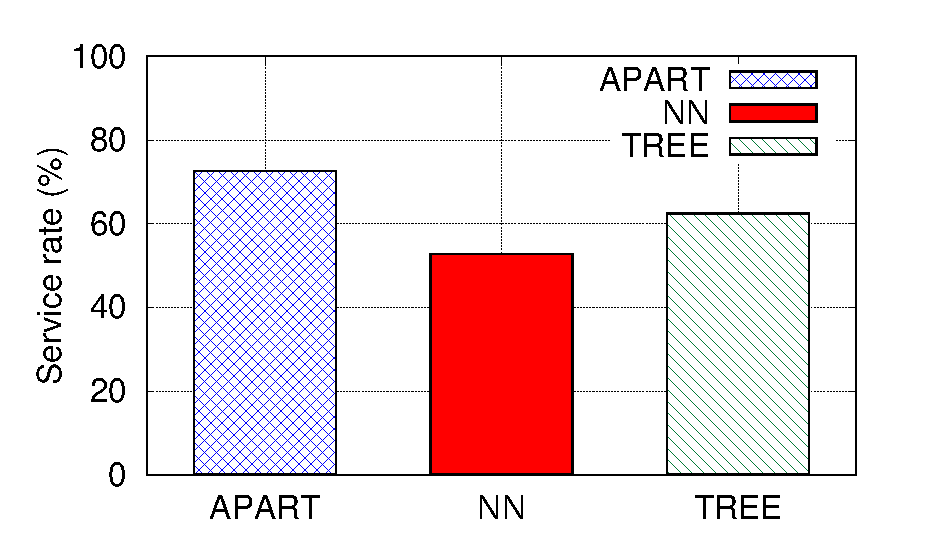
\includegraphics[width = 0.45\columnwidth]{fig/default_sr.eps}
    }
    \subfigure[\small{Driver Availability}]{
        \label{fig:availability}
        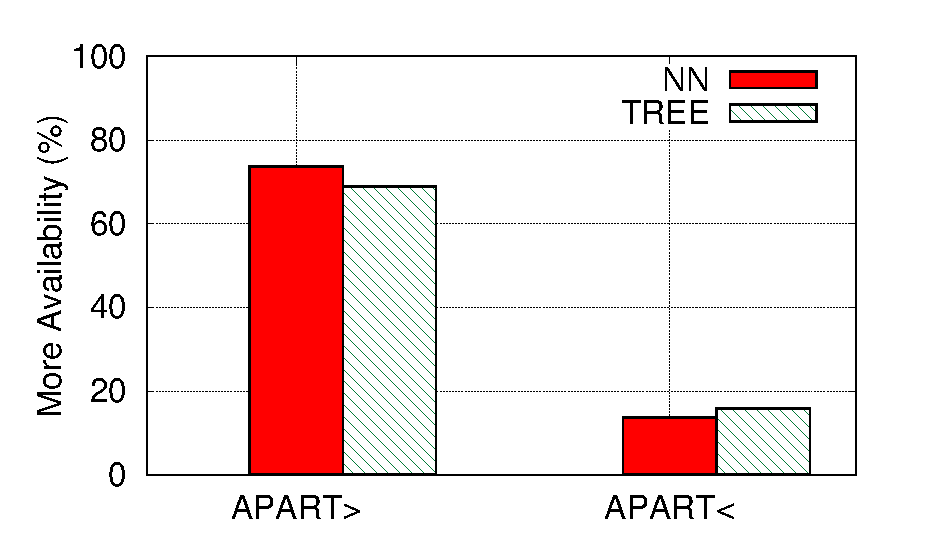
\includegraphics[width = 0.45\columnwidth]{fig/availability.eps}
    }
    \subfigure[\small{Revenue}]{
        \label{fig:default_rev}
        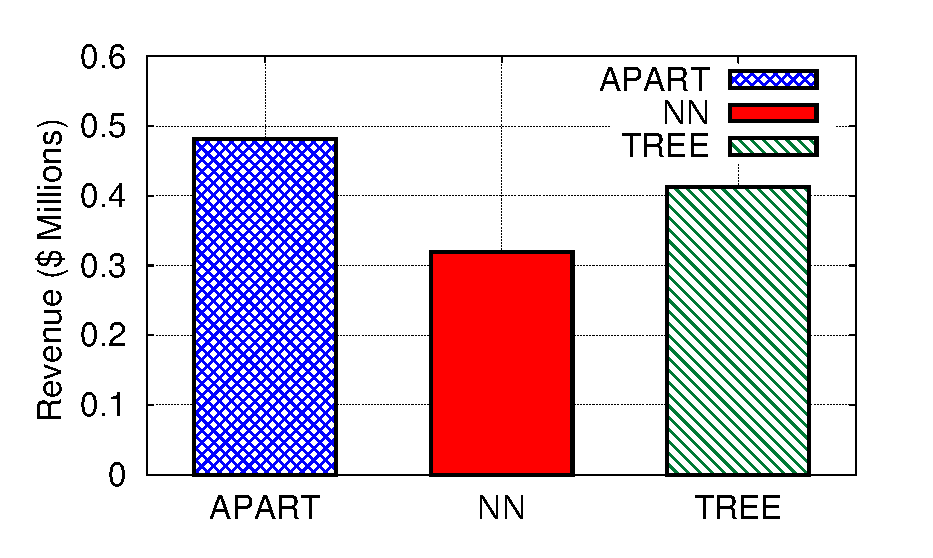
\includegraphics[width = 0.45\columnwidth]{fig/default_rev.eps}
    }
    \subfigure[\small{Response Time}]{
        \label{fig:default_rp}
        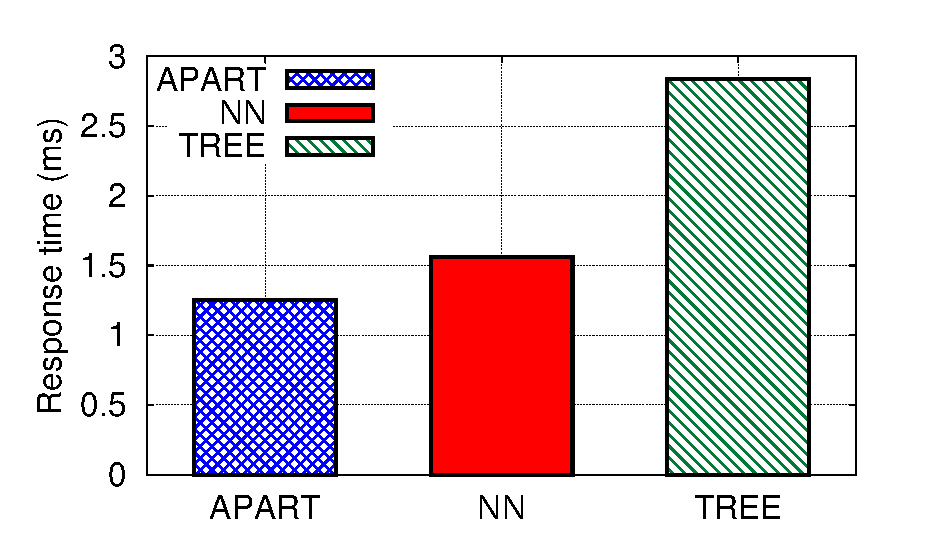
\includegraphics[width = 0.45\columnwidth]{fig/default_rp.eps}
    }
    \vspace{-0.15in}
    \caption{Comparing Algorithms with Default Values}
    \vspace{-5mm}
    \label{fig:defaults}
\end{figure*}

\subsection{Algorithm Comparison}

\subsubsection{Overall comparison}
In this section, we compare and analyze the performance of the three approaches using the default parameters in \cref{tab:params} with respect to service rate, generated revenue and response time.

As shown in \cref{fig:default_sr}, APART is able to serve more requests (i.e. higher service rate) compared to the other two approaches. For all three approaches we use the same set of requests and drivers for each iteration, which means all approaches start with the same configuration in the road network. However, each approach assigns riders to drivers differently and hence, after a while the dynamism of the network (i.e., location of the drivers on the road network) will be different in each algorithms. To understand the reason for higher service rate, for each incoming request, we also count the number of eligible workers (\cref{subsec:dispatch}). We say, the driver availability in algorithm $\mathcal{A}$ is higher than $\mathcal{B}$ with regard to request $r$, if during the simulation, more eligible drivers in algorithm $\mathcal{A}$ are available for $r$ compared to that of algorithm $\mathcal{B}$. \cref{fig:availability} shows the percentage of the requests for which APART has higher(/lower) driver availability compared to the other two approaches. The left two bars in \cref{fig:availability} show that for more than 60\% of the requests, APART has a higher driver availability compared to both NN and TREE. This means that APART engages drivers more effectively compared to NN and TREE and hence, is able to serve more requests.

Next, we compare the algorithms with regard to how much revenue they generate. \cref{fig:default_rev} shows APART generates almost 20\% and 50\% more revenue compared to TREE and NN, respectively. In \cref{sec:intro} we mentioned that the driver with minimum increase in his travel distance is not necessarily the most profitable driver. To verify this theory, when running TREE, for each incoming request (and after the algorithm chose the driver with least increase in traveled distance), we also check all eligible drivers to see which one generates the highest profit by serving the new request. We performed a similar check when running NN. Based on our observations, for 23\% of the requests, the driver chosen by TREE is different from the most profitable driver. This number for NN is 70\%. In \cref{subsec:expalgo} we explain, with implementation of TREE and NN the request is not assigned to a driver that cannot satisfy the monetary constraint. In other words, both approaches make sure by assigning a request to a driver, the platform provider does not loose money. If we relax this check for both approaches, in TREE, 5\% of the requests are assigned to drivers that loose money. This number is 40\% for NN.

The final metric we compare, is the average response time for processing a single request. As shown in \cref{fig:default_rp}, with the default setting, the processing time in TREE is almost twice the response time in APART. The reason is that although TREE utilizes a ``Kinetic Tree'' data structure which maintains the current available schedules to expedite the scheduling process, the server has to perform scheduling for eligible drivers sequentially while APART distributes the scheduling to the drivers. Nevertheless, with the default settings, all three approaches process the requests under 3ms which is acceptable for a real-time framework.

Following we vary different parameters based on \cref{tab:params} and evaluate the effect of each parameter on the same metrics.

\subsubsection{Service Rate}
In this set of experiments we compare the service rate of the three approaches. As shown in \cref{fig:sr}, all algorithms generate high service rates when the constraints are relaxed or there is high resource availability. However, under tight constraints or limited resources, APART outperforms the other two approaches by up to 20\%. In the previous section we showed how APART copes with the dynamism in the system better than the other two approaches.

\begin{figure}[h]
    \centering
    \subfigure[\small{Maximum Wait Time}]{
        \label{fig:mwt_sr}
        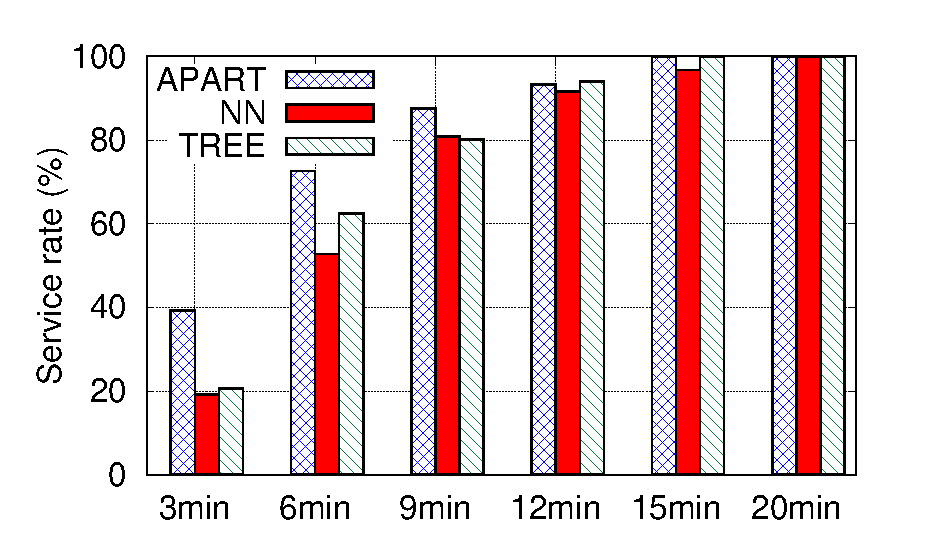
\includegraphics[width = 0.45\columnwidth]{fig/mwt_sr.eps}
    }
    \subfigure[\small{Number of Drivers}]{
        \label{fig:nd_sr}
        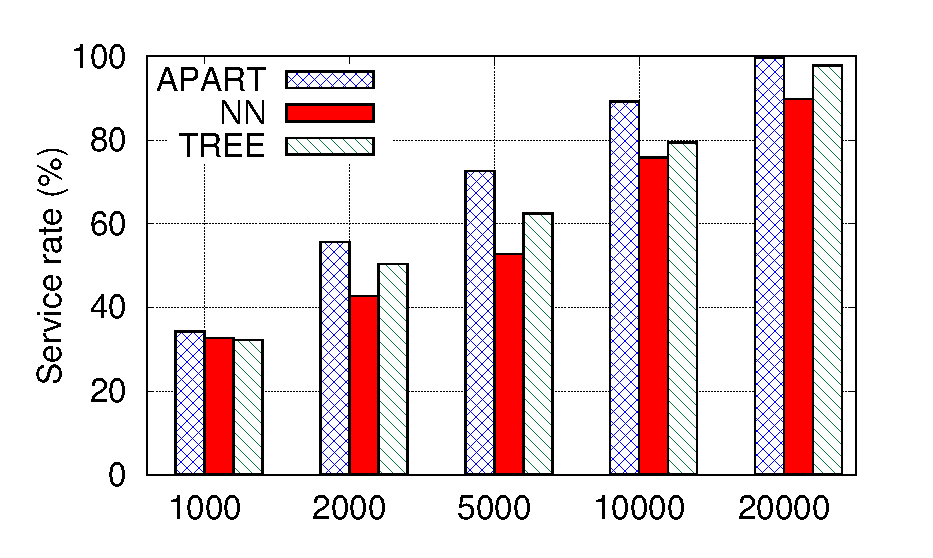
\includegraphics[width = 0.45\columnwidth]{fig/nd_sr.eps}
    }
    \subfigure[\small{Maximum Passengers}]{
        \label{fig:mp_sr}
        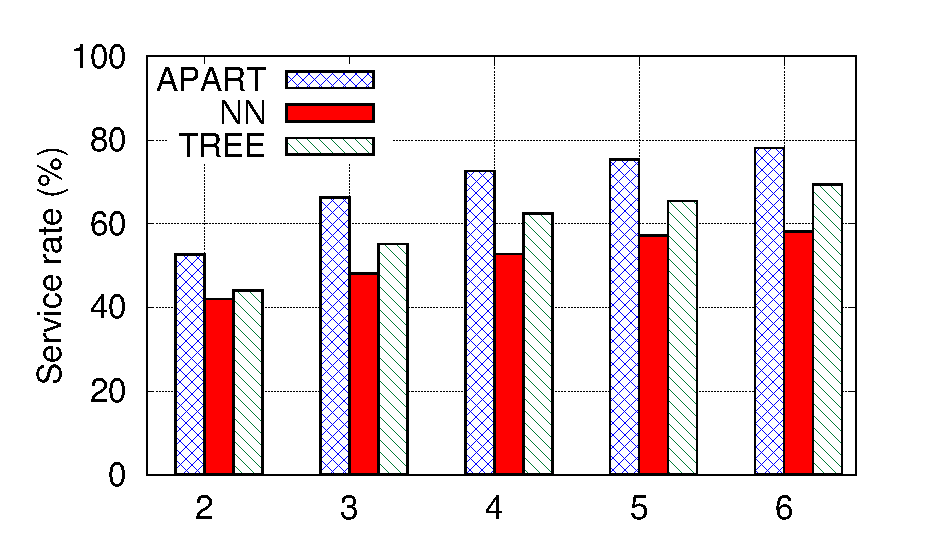
\includegraphics[width = 0.45\columnwidth]{fig/mp_sr.eps}
    }
    \subfigure[\small{Maximum Allowed Detour}]{
        \label{fig:mad_sr}
        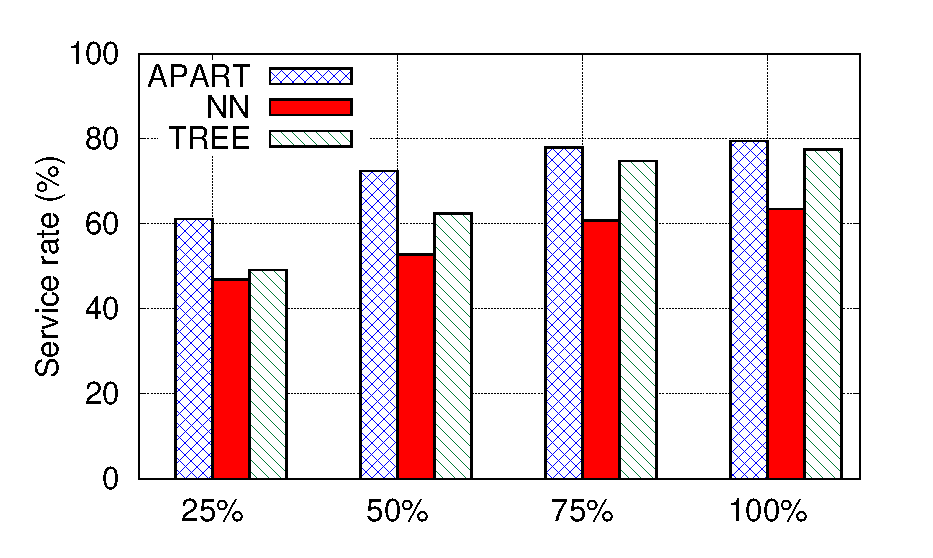
\includegraphics[width = 0.45\columnwidth]{fig/mad_sr.eps}
    }
    \vspace{-0.15in}
    \caption{Comparing Service Rate of the Algorithms}
    \label{fig:sr}
\end{figure}

\vspace{-5mm}
\subsubsection{Revenue}
As mentioned, the main objective of APART is to maximize the ride-sharing platform's revenue. In this experiment, we compare the generated revenue of each algorithm. Towards that end, we apply the pricing model explained in \cref{sec:pricing}. Here, we want to evaluate the effect of varying the parameters in \cref{tab:params} on the revenue and compare different algorithms. In \cref{subsec:pricingexp} we apply different pricing models to the algorithms and compare revenue under different pricing models.

\begin{figure}[h]
    \centering
    \subfigure[\small{Maximum Wait Time}]{
        \label{fig:mwt_rev}
        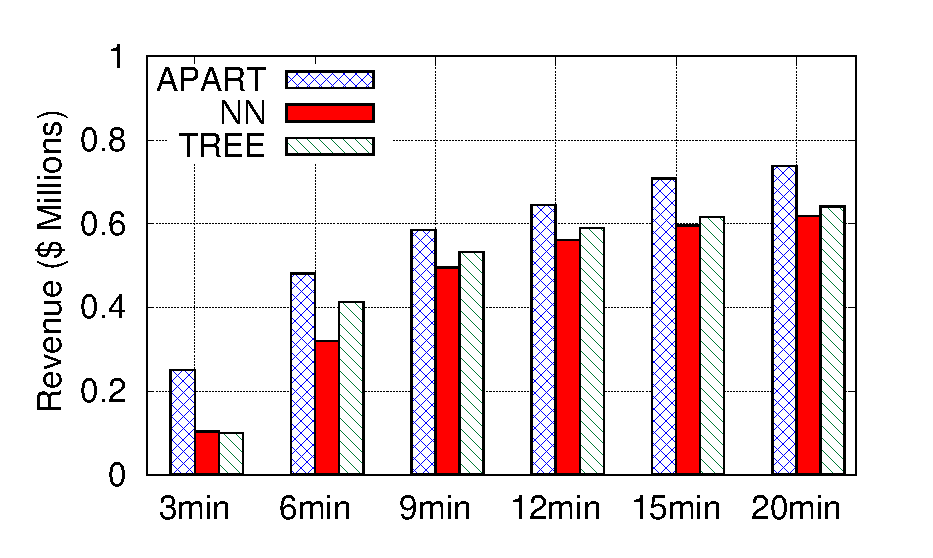
\includegraphics[width = 0.45\columnwidth]{fig/mwt_rev.eps}
    }
    \subfigure[\small{Number of Drivers}]{
        \label{fig:nd_rev}
        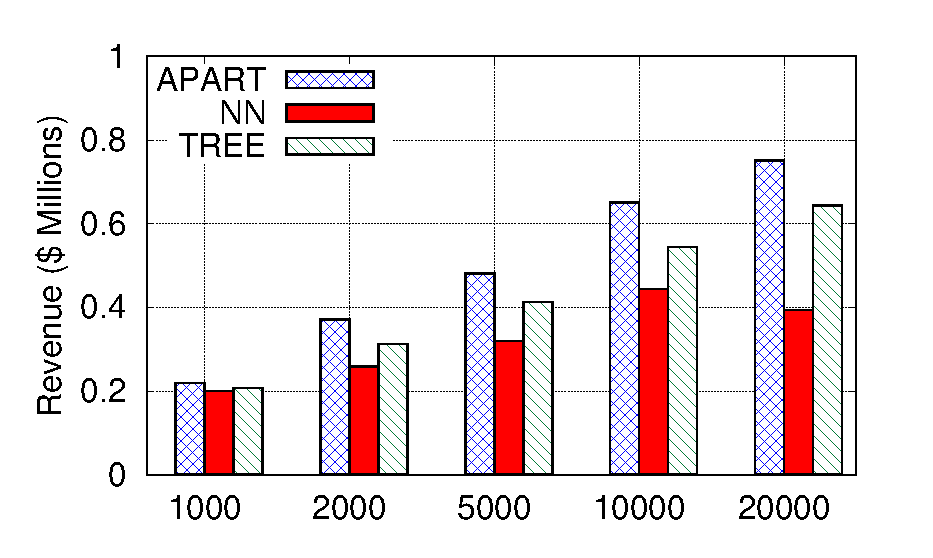
\includegraphics[width = 0.45\columnwidth]{fig/nd_rev.eps}
    }
    \subfigure[\small{Maximum Passengers}]{
        \label{fig:mp_rev}
        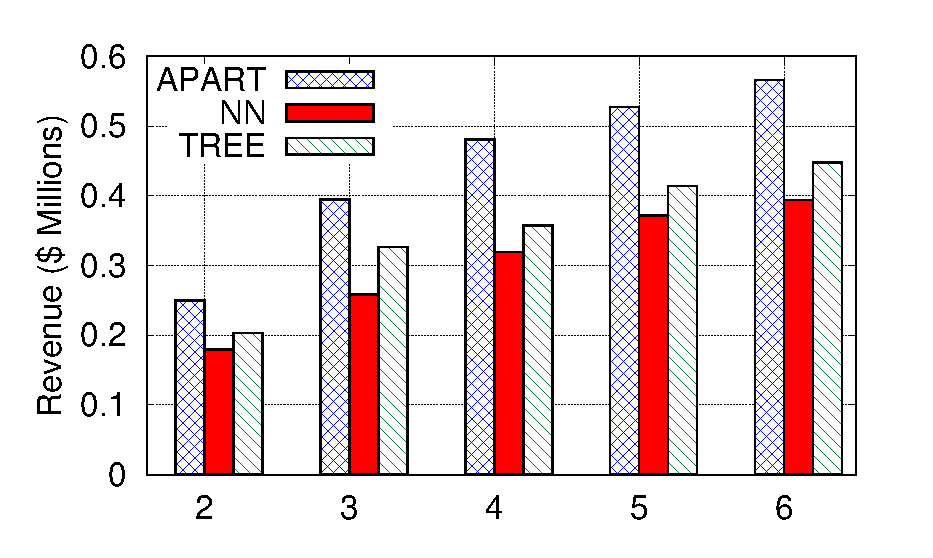
\includegraphics[width = 0.45\columnwidth]{fig/mp_rev.eps}
    }
    \subfigure[\small{Maximum Allowed Detour}]{
        \label{fig:mad_rev}
        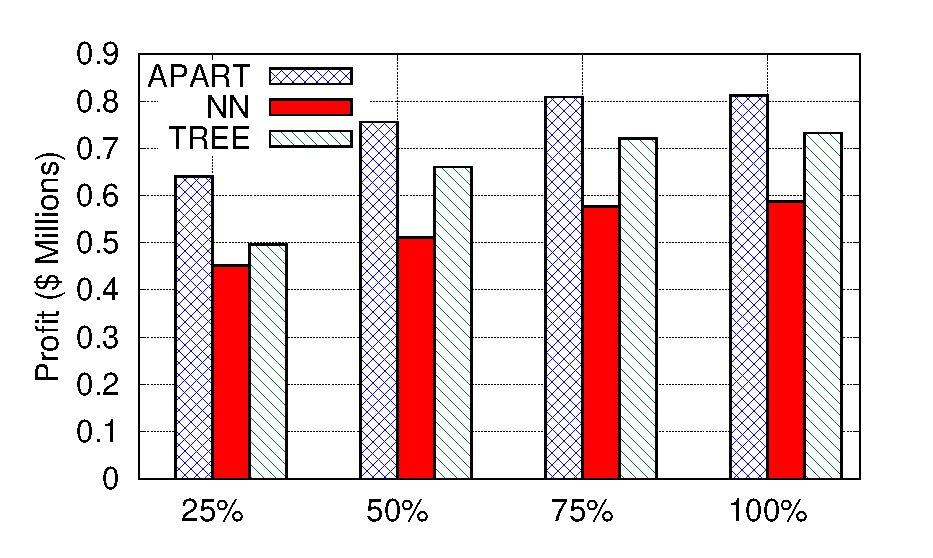
\includegraphics[width = 0.45\columnwidth]{fig/mad_rev.eps}
    }
    \vspace{-0.15in}
    \caption{Comparing Revenue of the Algorithms}
    \label{fig:rev}
\end{figure}

\cref{fig:rev} shows that regardless of the values of different parameters, APART generates more revenue than any other approaches. When we compare the results in \cref{fig:rev} with \cref{fig:sr}, even under configurations where all algorithms have the same service rate, APART manages to generate at least 10\% more revenue. The main reason for higher revenue is that APART is designed to make a \textit{price-aware} assignment, i.e., assign the request to a driver that generates the most profit. On the other hand, the TREE and NN algorithms were not designed to maximize revenue. As explained in \cref{sec:pricing}, the pricing models that are used in APART are designed such that the higher profits are not gained by scamming the riders.

\subsubsection{Response Time}
\label{subsec:exprp}

Similar to \cite{Ma13,Huang14}, APART instantly processes a request once it is submitted. In order to evaluate the scalability of our framework, our next set of experiments evaluate the response time of processing a single request. 

\begin{figure}[h]
    \centering
    \subfigure[\small{Maximum Wait Time}]{
        \label{fig:mwt_rp}
        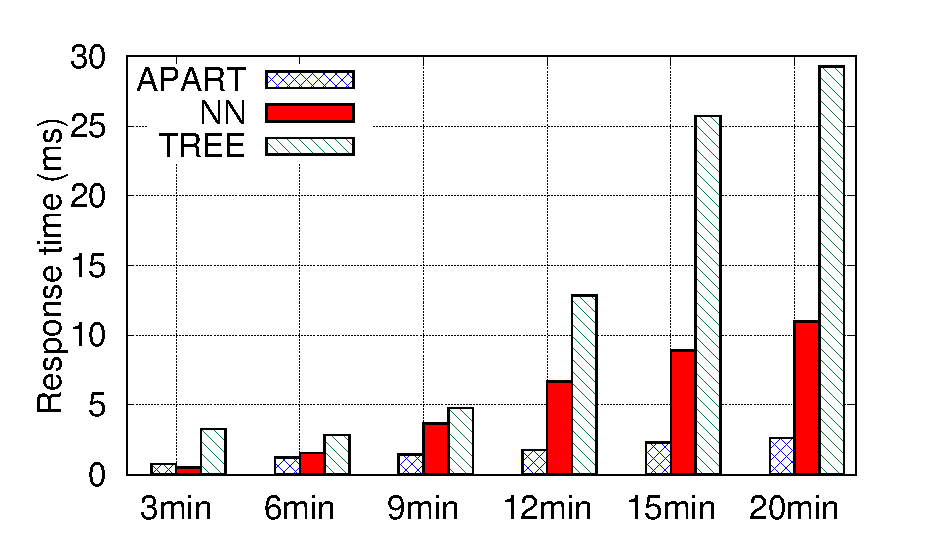
\includegraphics[width = 0.45\columnwidth]{fig/mwt_rp.eps}
    }
    \subfigure[\small{Number of Drivers}]{
        \label{fig:nd_rp}
        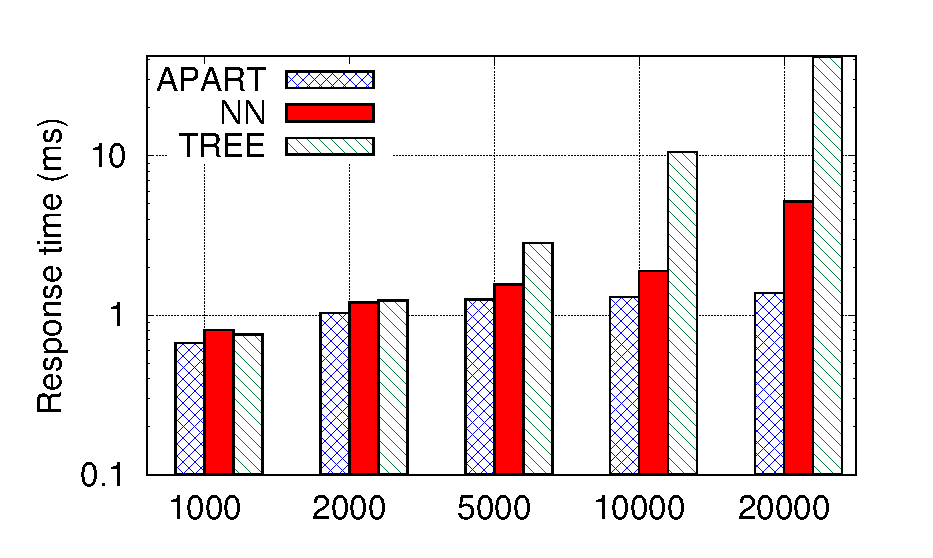
\includegraphics[width = 0.45\columnwidth]{fig/nd_rp.eps}
    }
    \subfigure[\small{Maximum Passengers}]{
        \label{fig:mp_rp}
        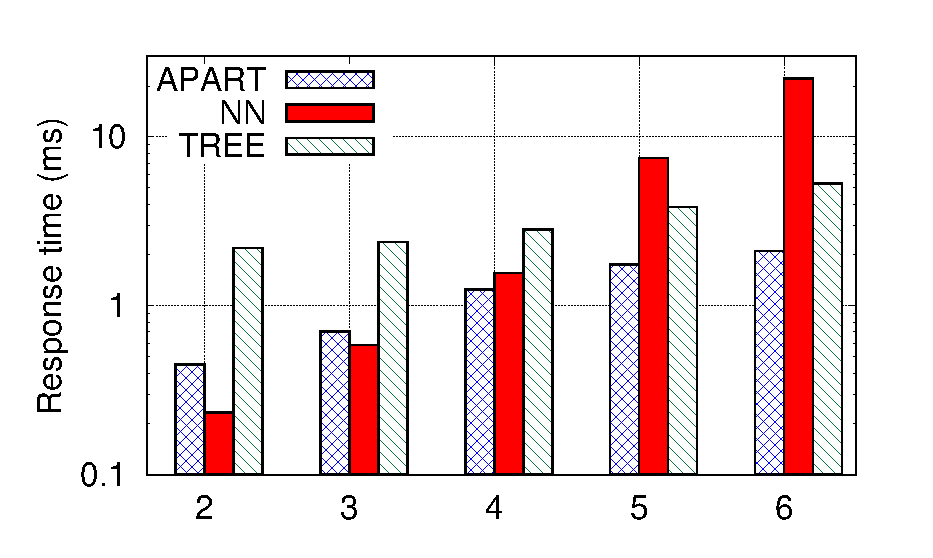
\includegraphics[width = 0.45\columnwidth]{fig/mp_rp.eps}
    }
    \subfigure[\small{Maximum Allowed Detour}]{
        \label{fig:mad_rp}
        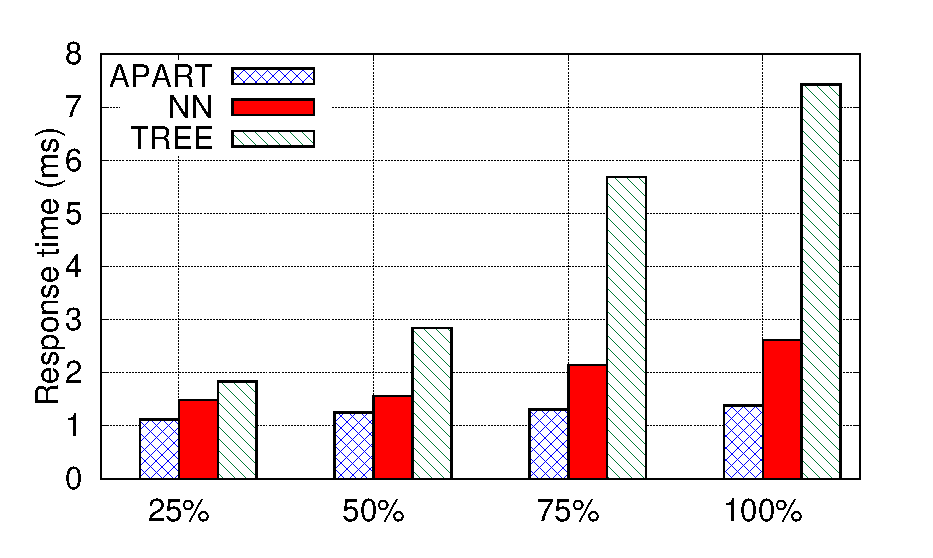
\includegraphics[width = 0.45\columnwidth]{fig/mad_rp.eps}
    }
    \vspace{-0.15in}
    \caption{Comparing Response Time of the Algorithms}
    \label{fig:rp}
\end{figure}

\vspace{-3mm}
\cref{fig:nd_rp} shows that when more drivers are added, the scalability of TREE suffers as it has to perform scheduling for a larger number of vehicles. On the other hand, due to the distributed nature of APART's auction-based approach, each driver does scheduling for itself and adding drivers does not affect the overall response time of APART as much. In \cref{fig:mp_rp} we observe that although APART's response time does not go beyond 5ms, TREE handles the increase in maximum passengers better due to the Kinetic Tree structure implementation \cite{Huang14}. The reason for NN's poor performance is that it has to perform scheduling computation sequentially, for possibly multiple drivers. Finally, in \cref{fig:mwt_rp} and \cref{fig:mad_rp} we conclude that for relaxed constraints, the response time of TREE increases up to 4 times higher than that of APART. The main reason is that the Kinetic Tree structure keeps track of all valid orders of requests that are assigned to a driver. As we relax the constraints, the number of feasible permutations of the requests increases which makes the size of the Kinetic Tree larger and updates become more expensive. This in turn increases the response time. \cref{fig:rp} shows unlike the other two approaches, APART's scalability does not suffer by varying different parameters of the framework.

\subsection{Comparing Different Pricing Models}
\label{subsec:pricingexp}

In this section, we evaluate the effect of the pricing model. First we show the importance of designing a fair pricing model. We utilize the three approaches with the model in \cite{Ma13} and show how some riders may suffer by participating in ride-sharing. Subsequently, we perform some experiments utilizing the pricing model in \cite{Ma15} and show that as a result of price-aware assignments, regardless of the model, APART generates more revenue for the platform provider. Finally, we show the flexibility that profiles provide for the users. 

\cref{fig:fairness} shows the result of utilizing the pricing model in \cite{Ma13}. Based on this pricing model, the driver's income is:

\vspace{-2mm}
\begin{center}
$c.d_1 + (1+\alpha).c.d_2$
\end{center}
\vspace{-2mm}

\noindent where $d_1$ is the distance the driver had only one rider on-board, $d_2$ is the total distance the driver had more than one rider on-board and $c$ is some predefined constant. $\alpha$ takes a value between 0 and 1 which determines the increase in the driver's income for serving more than one rider. As we show in \cref{fig:saved}, by participating in ride-sharing, the majority of riders save money (pay less as compared to riding alone). \cref{fig:saved} supports the claim in \cite{Ma13} that on average riders will save money. However, \cref{fig:lost} shows that regardless of what algorithm is used, up to 10\% of riders pay more by participating in ride-sharing which is not acceptable. The reason is that, riders have to pay even for detours. Even though riders split the fare on detours, if detours are sufficiently long, even carpooling riders loose money.

\begin{figure}[h!]
	\centering
    \subfigure[\small{Rider's that Saved Money}]{
        \label{fig:saved}
        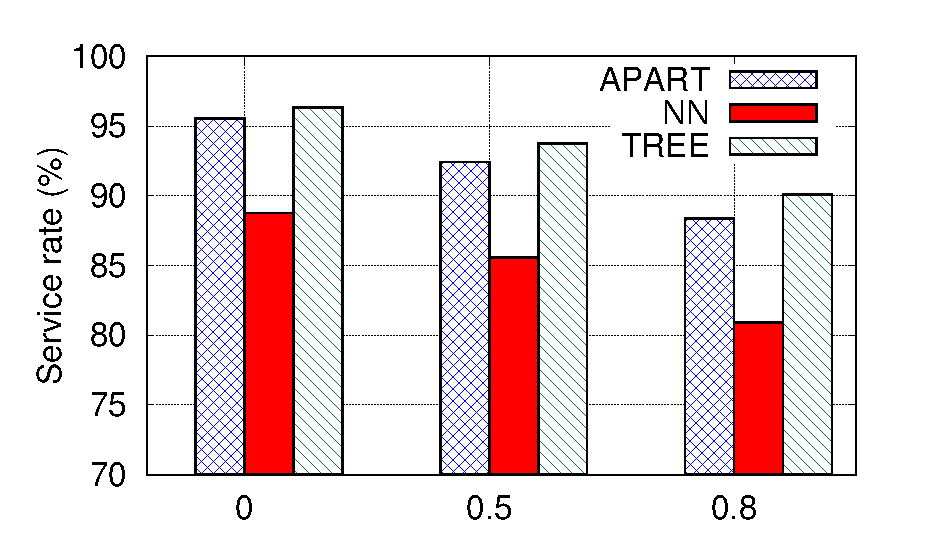
\includegraphics[width = 0.45\columnwidth]{fig/saved.eps}
    }
    \subfigure[\small{Rider's that Lost Money}]{
        \label{fig:lost}
        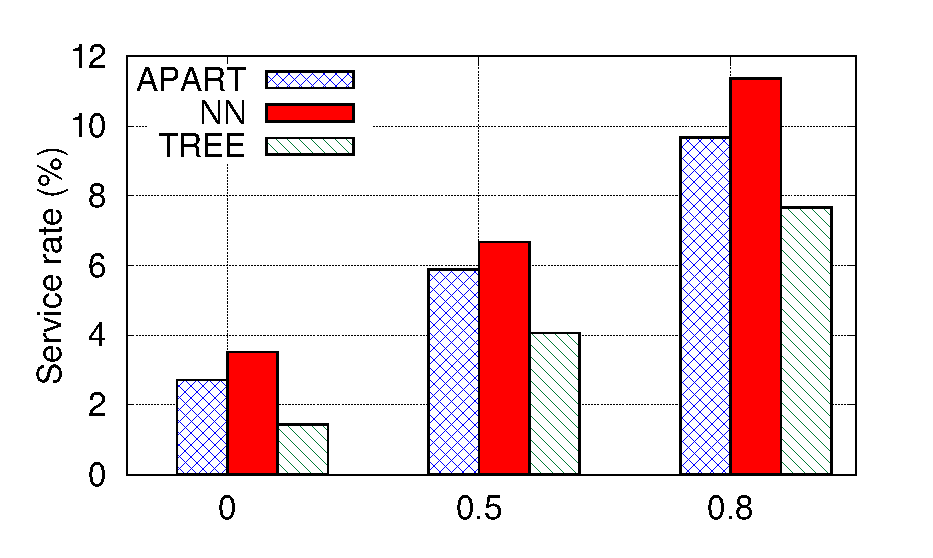
\includegraphics[width = 0.45\columnwidth]{fig/lost.eps}
    }
    \vspace{-0.15in}
    \caption{Fairness of Pricing Models}
    \label{fig:fairness}
\end{figure}

\vspace{-3mm}
In the next set of experiments, we apply the model in \cite{Ma15} and evaluate the performance of APART and TREE. In this model, riders get compensated for any detour incurred in their trip. The amount of compensation is based on the new rider's fare and the length of a rider's detour compared with the detour of other riders on the vehicle. Because the algorithm in \cite{Ma15} is similar to TREE, we only compared APART with TREE. \cref{fig:tkde_sr} shows that APART provides a slightly higher service rate than TREE. However, due to assigning the riders to the most profitable drivers, APART ends up generating 10\% more revenue.

\begin{figure}[h]
	\centering
    \subfigure[\small{Service Rate}]{
        \label{fig:tkde_sr}
        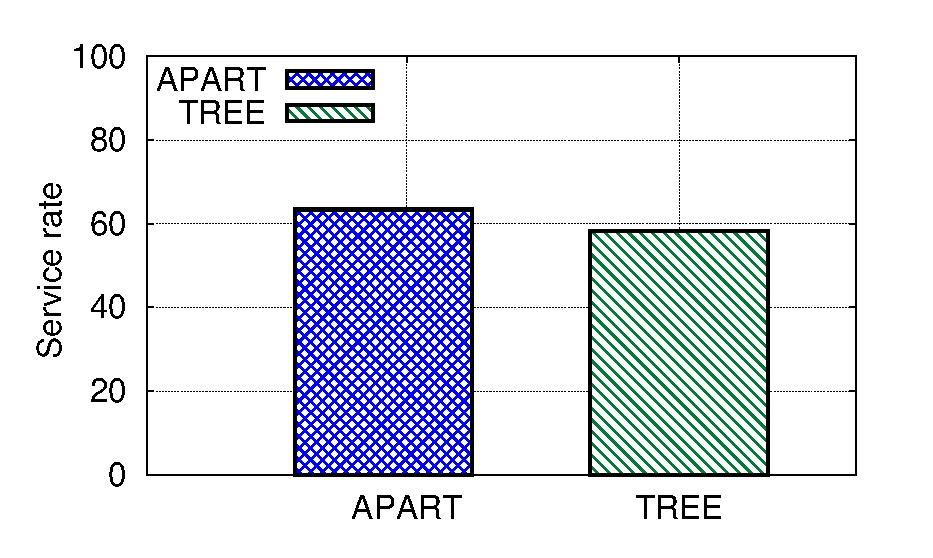
\includegraphics[width = 0.45\columnwidth]{fig/tkde_sr.eps}
    }
    \subfigure[\small{Revenue}]{
        \label{fig:tkde_rev}
        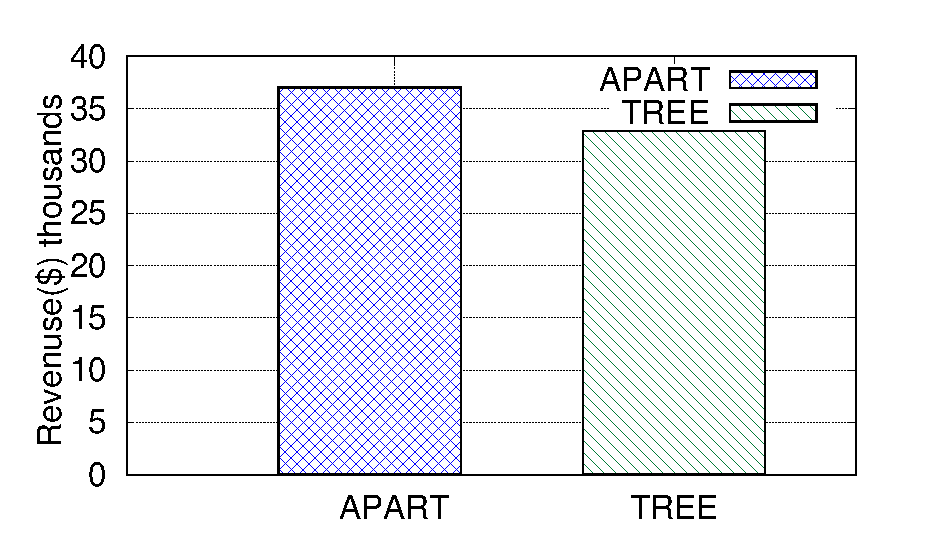
\includegraphics[width = 0.45\columnwidth]{fig/tkde_rev.eps}
    }
    \vspace{-0.15in}
    \caption{Effect of Applying an Arbitrary Pricing Model}
    \vspace{-2mm}
    \label{fig:tkde}
\end{figure}

In \cref{sec:pricing}, we mentioned by setting their profiles, users can configure APART to make assignments the way they find desirable. In the last set of our experiments, we use two different configurations to represent the riders' profiles. First, we set the riders' profiles to $f_T(\Delta d_r) = \frac{1}{(\Delta d_r + 1)}$. Such profile is suitable for a rider who wants to minimize his detour and is willing to share a ride only if the detour is short. Since the rider sets \textbf{Tight} constraints we show this profile by $f_T$. In the second iteration, we set the profile of the riders to $f_R(\Delta d_r) = 1 -  (\frac{\Delta d_r}{max \delta})$. This profile is more \textbf{Relaxed} (hence, $f_R$) and it is expected that more riders share a trip. \cref{fig:quality} shows the result of utilizing APART and TREE with $f_T$ and $f_R$. Since TREE does not make price-aware assignments, the results in both iterations were the same. However, as we observe with APART\_T, almost 10\% fewer riders ended up sharing a ride while on average they only observed 6-7\% increase in their trips. On the other hand, with APART\_R, almost every rider shares a ride and the average increase in their trip was almost 20\%. An interesting observation in \cref{fig:quality} is that with APART\_R, more riders share a ride compared to TREE while their average detour was still less.

\begin{figure}[h]
	\centering
    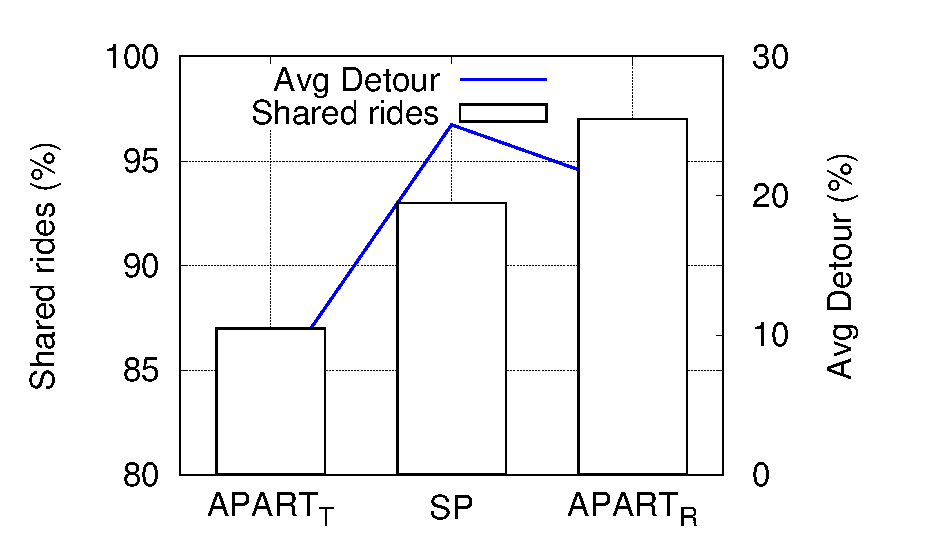
\includegraphics[width = 0.65\columnwidth]{fig/quality.eps}
    \vspace{-0.15in}
    \caption{Effect of Profiles}
    \label{fig:quality}
\end{figure}
\vspace{-0.1in}

In conclusion, APART is agnostic of the price model and is able to generate more profit. In addition, APART supports different types of riders' expectations by adjusting the profiles.